\documentclass[onlymath]{beamer}
% \documentclass[onlymath,handout]{beamer}

% Macros used by all lectures, but not necessarily by excercises

%%% General setup and dependencies:

% \usetheme[ddcfooter,nosectionnum]{tud}
\usetheme[nosectionnum,pagenum,noheader]{tud}
% \usetheme[nosectionnum,pagenum]{tud}

% Increase body font size to a sane level:
\let\origframetitle\frametitle
% \renewcommand{\frametitle}[1]{\origframetitle{#1}\normalsize}
\renewcommand{\frametitle}[1]{\origframetitle{#1}\fontsize{10pt}{13.2}\selectfont}
\setbeamerfont{itemize/enumerate subbody}{size=\small} % tud defaults to scriptsize!
\setbeamerfont{itemize/enumerate subsubbody}{size=\small}
% \setbeamerfont{normal text}{size=\small}
% \setbeamerfont{itemize body}{size=\small}

\renewcommand{\emph}[1]{\textbf{#1}}

\def\arraystretch{1.3}% Make tables even less cramped vertically

\usepackage[ngerman]{babel}
\usepackage[utf8]{inputenc}
\usepackage[T1]{fontenc}

%\usepackage{graphicx}
\usepackage[export]{adjustbox} % loads graphicx
\usepackage{import}
\usepackage{stmaryrd}
\usepackage[normalem]{ulem} % sout command
% \usepackage{times}
\usepackage{txfonts}
\usepackage{array}

% \usepackage[perpage]{footmisc} % reset footnote counter on each page -- fails with beamer (footnotes gone)
\usepackage{perpage}  % reset footnote counter on each page
\MakePerPage{footnote}

\usepackage{tikz}
\usetikzlibrary{arrows,positioning,decorations.pathreplacing}
% Inspired by http://www.texample.net/tikz/examples/hand-drawn-lines/
\usetikzlibrary{decorations.pathmorphing}
\pgfdeclaredecoration{penciline}{initial}{
    \state{initial}[width=+\pgfdecoratedinputsegmentremainingdistance,
    auto corner on length=1mm,]{
        \pgfpathcurveto%
        {% From
            \pgfqpoint{\pgfdecoratedinputsegmentremainingdistance}
                      {\pgfdecorationsegmentamplitude}
        }
        {%  Control 1
        \pgfmathrand
        \pgfpointadd{\pgfqpoint{\pgfdecoratedinputsegmentremainingdistance}{0pt}}
                    {\pgfqpoint{-\pgfdecorationsegmentaspect
                     \pgfdecoratedinputsegmentremainingdistance}%
                               {\pgfmathresult\pgfdecorationsegmentamplitude}
                    }
        }
        {%TO
        \pgfpointadd{\pgfpointdecoratedinputsegmentlast}{\pgfpoint{1pt}{1pt}}
        }
    }
    \state{final}{}
}
\tikzset{handdrawn/.style={decorate,decoration=penciline}}
\tikzset{every shadow/.style={fill=none,shadow xshift=0pt,shadow yshift=0pt}}
% \tikzset{module/.append style={top color=\col,bottom color=\col}}

% Use to make Tikz attributes with Beamer overlays
% http://tex.stackexchange.com/a/6155
\tikzset{onslide/.code args={<#1>#2}{%
  \only<#1| handout:0>{\pgfkeysalso{#2}}
}}
\tikzset{onslideprint/.code args={<#1>#2}{%
  \only<#1>{\pgfkeysalso{#2}}
}}

%%% Title -- always set this first

\newcommand{\defineTitle}[3]{
	\newcommand{\lectureindex}{#1}
	\title{Theoretische Informatik und Logik}
	\subtitle{\href{\lectureurl}{#1. Vorlesung: #2}}
	\author{\href{https://iccl.inf.tu-dresden.de/web/Markus_Kr\%C3\%B6tzsch}{Markus Kr\"{o}tzsch}\\[1ex]Lehrstuhl Wissensbasierte Systeme}
	\date{#3}
	\datecity{TU Dresden}
% 	\institute{CC-By 3.0, sofern keine anderslautenden Bildrechte angegeben sind}
}

%%% Table of contents:

\RequirePackage{ifthen}

\newcommand{\highlight}[2]{%
	\ifthenelse{\equal{#1}{\lectureindex}}{\alert{#2}}{#2}%
}

\def\myspace{-0.7ex}
\newcommand{\printtoc}{
\begin{tabular}{r@{$\quad$}l}
\highlight{1}{1.} & \highlight{1}{Willkommen/Einleitung formale Sprachen}\\[\myspace]
\highlight{2}{2.} & \highlight{2}{Grammatiken und die Chomsky-Hierarchie}\\[\myspace]
\highlight{3}{3.} & \highlight{3}{Endliche Automaten}\\[\myspace]
\highlight{4}{4.} & \highlight{4}{Complexity of FO query answering}\\[\myspace]
\highlight{5}{5.} & \highlight{5}{Conjunctive queries}\\[\myspace]
\highlight{6}{6.} & \highlight{6}{Tree-like conjunctive queries}\\[\myspace]
\highlight{7}{7.} & \highlight{7}{Query optimisation}\\[\myspace]
\highlight{8}{8.} & \highlight{8}{Conjunctive Query Optimisation / First-Order~Expressiveness}\\[\myspace]
\highlight{9}{9.} & \highlight{9}{First-Order~Expressiveness / Introduction to Datalog}\\[\myspace]
\highlight{10}{10.} & \highlight{10}{Expressive Power and Complexity of Datalog}\\[\myspace]
\highlight{11}{11.} & \highlight{11}{Optimisation and Evaluation of Datalog}\\[\myspace]
\highlight{12}{12.} & \highlight{12}{Evaluation of Datalog (2)}\\[\myspace]
\highlight{13}{13.} & \highlight{13}{Graph Databases and Path Queries}\\[\myspace]
\highlight{14}{14.} & \highlight{14}{Outlook: database theory in practice}
\end{tabular}
}

\newcommand{\overviewslide}{%
\begin{frame}\frametitle{Overview}
\printtoc
\medskip

Siehe \href{\lectureurl}{course homepage [$\Rightarrow$ link]} for more information and materials
\end{frame}
}

%%% Colours:
\usepackage{xcolor,colortbl}
\definecolor{redhighlights}{HTML}{FFAA66}
\definecolor{lightblue}{HTML}{55AAFF}
\definecolor{lightred}{HTML}{FF5522}
\definecolor{lightpurple}{HTML}{DD77BB}
\definecolor{lightgreen}{HTML}{55FF55}
\definecolor{darkred}{HTML}{CC4411}
\definecolor{darkblue}{HTML}{176FC0}%{1133AA}
\definecolor{nightblue}{HTML}{2010A0}%{1133AA}
\definecolor{alert}{HTML}{176FC0}
\definecolor{darkgreen}{HTML}{36AB14}
\definecolor{strongyellow}{HTML}{FFE219}
\definecolor{devilscss}{HTML}{666666}

\newcommand{\redalert}[1]{\textcolor{darkred}{#1}}

%%% Slide layout commands:

\newcommand{\sectionSlide}[1]{
\frame{\begin{center}
\LARGE
#1
\end{center}}
}
\newcommand{\sectionSlideNoHandout}[1]{
\frame<handout:0>{\begin{center}
\LARGE
#1
\end{center}}
}

\newcommand{\mydualbox}[3]{%
 \begin{minipage}[t]{#1}
 \begin{beamerboxesrounded}[upper=block title,lower=block body,shadow=true]%
    {\centering\usebeamerfont*{block title}#2}%
    \raggedright%
    \usebeamerfont{block body}
%     \small
    #3%
  \end{beamerboxesrounded}
  \end{minipage}
}
%
\newcommand{\myheaderbox}[2]{%
 \begin{minipage}[t]{#1}
 \begin{beamerboxesrounded}[upper=block title,lower=block title,shadow=true]%
    {\centering\usebeamerfont*{block title}\rule{0pt}{2.6ex} #2}%
  \end{beamerboxesrounded}
  \end{minipage}
}

\newcommand{\mycontentbox}[2]{%
 \begin{minipage}[t]{#1}%
 \begin{beamerboxesrounded}[upper=block body,lower=block body,shadow=true]%
    {\centering\usebeamerfont*{block body}\rule{0pt}{2.6ex}#2}%
  \end{beamerboxesrounded}
  \end{minipage}
}

\newcommand{\mylcontentbox}[2]{%
 \begin{minipage}[t]{#1}%
 \begin{beamerboxesrounded}[upper=block body,lower=block body,shadow=true]%
    {\flushleft\usebeamerfont*{block body}\rule{0pt}{2.6ex}#2}%
  \end{beamerboxesrounded}
  \end{minipage}
}

% label=180:{\rotatebox{90}{{\footnotesize\textcolor{darkgreen}{Beispiel}}}}
% \hspace{-8mm}\ghost{\raisebox{-7mm}{\rotatebox{90}{{\footnotesize\textcolor{darkgreen}{Beispiel}}}}}\hspace{8mm}
\newcommand{\examplebox}[1]{%
	\begin{tikzpicture}[decoration=penciline, decorate]
		\pgfmathsetseed{1235}
		\node (n1) [decorate,draw=darkgreen, fill=darkgreen!10,thick,align=left,text width=\linewidth, inner ysep=2mm, inner xsep=2mm] at (0,0) {#1};
% 		\node (n2) [align=left,text width=\linewidth,inner sep=0mm] at (n1.92) {{\footnotesize\raisebox{3mm}{\textcolor{darkgreen}{Beispiel}}}};
% 		\node (n2) [decorate,draw=darkgreen, fill=darkgreen!10,thick, align=left,text width=\linewidth,inner sep=2mm] at (n1.90) {{\footnotesize\raisebox{0mm}{\textcolor{darkgreen}{Beispiel}}}};
	\end{tikzpicture}%
}%

\newcommand{\codebox}[1]{%
	\begin{tikzpicture}[decoration=penciline, decorate]
		\pgfmathsetseed{1236}
		\node (n1) [decorate,draw=strongyellow, fill=strongyellow!10,thick,align=left,text width=\linewidth, inner ysep=2mm, inner xsep=2mm] at (0,0) {#1};
	\end{tikzpicture}%
}%

\newcommand{\defbox}[1]{%
	\begin{tikzpicture}[decoration=penciline, decorate]
		\pgfmathsetseed{1237}
		\node (n1) [decorate,draw=darkred, fill=darkred!10,thick,align=left,text width=\linewidth, inner ysep=2mm, inner xsep=2mm] at (0,0) {#1};
	\end{tikzpicture}%
}%

\newcommand{\theobox}[1]{%
	\begin{tikzpicture}[decoration=penciline, decorate]
		\pgfmathsetseed{1240}
		\node (n1) [decorate,draw=darkblue, fill=darkblue!10,thick,align=left,text width=\linewidth, inner ysep=2mm, inner xsep=2mm] at (0,0) {#1};
	\end{tikzpicture}%
}%

\newcommand{\anybox}[2]{%
	\begin{tikzpicture}[decoration=penciline, decorate]
		\pgfmathsetseed{1240}
		\node (n1) [decorate,draw=#1, fill=#1!10,thick,align=left,text width=\linewidth, inner ysep=2mm, inner xsep=2mm] at (0,0) {#2};
	\end{tikzpicture}%
}%


\newsavebox{\mybox}%
\newcommand{\doodlebox}[2]{%
\sbox{\mybox}{#2}%
	\begin{tikzpicture}[decoration=penciline, decorate]
		\pgfmathsetseed{1238}
		\node (n1) [decorate,draw=#1, fill=#1!10,thick,align=left,inner sep=1mm] at (0,0) {\usebox{\mybox}};
	\end{tikzpicture}%
}%


\defineTitle{17}{Funktionen und Normalformen}{21. Juni 2017}

\begin{document}

\maketitle

\begin{frame}\frametitle{Resolution für Prädikatenlogik}

Ein konkreter Algorithmus zum logischen Schließen:
\begin{enumerate}[(1)]
\item \alert{Logische Konsequenz auf Unerfüllbarkeit reduzieren}
\item \alert{Formeln in Klauselform umwandeln}
	\begin{itemize}
	\item Formel bereinigen
	\item Negationsnormalform bilden
	\item \textcolor{devilscss}{Pränexform bilden}
	\item \textcolor{devilscss}{Skolemform bilden}
	\item \textcolor{devilscss}{Konjunktive Normalform bilden}
	\end{itemize}
\item \alert{Resolutionsverfahren anwenden}
	\begin{itemize}
	\item \textcolor{devilscss}{Unifikation zum Finden passender Klauseln}
	\item \textcolor{devilscss}{Bilden von Resolventen bis zur Terminierung}
	\end{itemize}
\end{enumerate}

\end{frame}


\begin{frame}\frametitle{Bereinigte Formeln}

\defbox{Eine Formel $F$ ist \redalert{bereinigt} wenn sie die folgenden beiden Eigenschaften hat:
\begin{enumerate}[(1)]
\item Keine Variable in $F$ kommt sowohl frei als auch gebunden vor
\item Keine Variable in $F$ wird in mehr als einem Quantor gebunden
\end{enumerate}}

Man kann jede Formel leicht durch Umbenennung gebundener Variablen
bereinigen.

\examplebox{Beispiel: Die Formel
\[ \forall y.p(x,y)\to \exists x.(r(y,x)\wedge\forall y.q(x,y)) \]
kann wie folgt bereinigt werden:
\[ \forall y.p(x,y)\to \exists z.(r(y,z)\wedge\forall v.q(z,v)) \]
}

\end{frame}

\begin{frame}\frametitle{Beispiel: Logelei}

In Vorlesung 14 betrachteten wir den Fall, dass alle Einwohner einer Insel sagen,
"`Auf dieser Insel haben alle den gleichen Typ."'\bigskip

Dies entspricht der Theorie aus folgenden Sätzen:
\begin{itemize}
\item "`Jeder Einwohner ist entweder Wahrheitssager oder Lügner."'\\
	$\alert{\forall x.\big((W(x)\wedge\neg L(x))\vee (L(x)\wedge\neg W(x))\big)}$
\item Lebt auf der Insel ein Wahrheitssager, dann stimmt die Behauptung:\\
	$\alert{\exists x.W(x)\to(\forall x.W(x) \vee \forall x.L(x))}$
\item Lebt auf der Insel ein Lügner, dann ist die Behauptung falsch:\\
	$\alert{\exists x.L(x)\to\neg(\forall x.W(x) \vee \forall x.L(x))}$
\end{itemize}\medskip\pause

Diese Theorie ist darstellbar als Konjunktion:
\begin{align*}
& \forall x.\big((W(x)\wedge\neg L(x))\vee (L(x)\wedge\neg W(x))\big)\\
{}\wedge{} & \big(\exists x.W(x)\to(\forall x.W(x) \vee \forall x.L(x))\big) \\
{}\wedge{} & \big(\exists x.L(x)\to\neg(\forall x.W(x) \vee \forall x.L(x))\big)
\end{align*}


\end{frame}

\begin{frame}\frametitle{Beispiel: Bereinigung}

\begin{align*}
& \forall x.\big((W(x)\wedge\neg L(x))\vee (L(x)\wedge\neg W(x))\big)\\
{}\wedge{} & \big(\exists x.W(x)\to(\forall x.W(x) \vee \forall x.L(x))\big) \\
{}\wedge{} & \big(\exists x.L(x)\to\neg(\forall x.W(x) \vee \forall x.L(x))\big)
\end{align*}\pause

Wir bereinigen die Formel, indem wir alle gebundenen Variablen umbenennen:
\begin{align*}
& \forall x_1.\big((W(x_1)\wedge\neg L(x_1))\vee (L(x_1)\wedge\neg W(x_1))\big)\\
{}\wedge{} & \big(\exists x_2.W(x_2)\to(\forall x_3.W(x_3) \vee \forall x_4.L(x_4))\big) \\
{}\wedge{} & \big(\exists x_5.L(x_5)\to\neg(\forall x_6.W(x_6) \vee \forall x_7.L(x_7))\big)
\end{align*}

\end{frame}

\newcommand{\hi}[2]{\textcolor{white}{\textcolor<#1>{purple}{\underline{\textcolor{HKS41K100}{#2}}}}}
\begin{frame}\frametitle{Beispiel: Negationsnormalform}


Jetzt bilden wir die NNF:
{\footnotesize
\[\begin{array}{rl}
& \forall x_1.\big((W(x_1)\wedge\neg L(x_1))\vee (L(x_1)\wedge\neg W(x_1))\big)\\
& {}\wedge{}  \hi{2-}{\big(\exists x_2.W(x_2)\textcolor{purple}{{}\to{}}(\forall x_3.W(x_3) \vee \forall x_4.L(x_4))\big)}\\
& {}\wedge{}  \hi{2-}{\big(\exists x_5.L(x_5)\textcolor{purple}{{}\to{}}\neg(\forall x_6.W(x_6) \vee \forall x_7.L(x_7))\big)}\\\pause\pause
%
{}\equiv{} & \forall x_1.\big((W(x_1)\wedge\neg L(x_1))\vee (L(x_1)\wedge\neg W(x_1))\big)\\
& {}\wedge{}  \big(\hi{4-}{\textcolor{purple}{{}\neg{}}\exists x_2.W(x_2)}\vee(\forall x_3.W(x_3) \vee \forall x_4.L(x_4))\big)\\
& {}\wedge{}  \big(\hi{4-}{\textcolor{purple}{{}\neg{}}\exists x_5.L(x_5)}\vee\hi{4-}{\textcolor{purple}{{}\neg{}}(\forall x_6.W(x_6) \vee \forall x_7.L(x_7))}\big)\\\pause\pause
%
{}\equiv{} & \forall x_1.\big((W(x_1)\wedge\neg L(x_1))\vee (L(x_1)\wedge\neg W(x_1))\big)\\
& {}\wedge{}  \big(\forall x_2.\neg W(x_2)\vee(\forall x_3.W(x_3) \vee \forall x_4.L(x_4))\big)\\
& {}\wedge{}  \big(\forall x_5.\neg L(x_5)\vee(\hi{6-}{\textcolor{purple}{{}\neg{}}\forall x_6. W(x_6)} \wedge \hi{6-}{\textcolor{purple}{{}\neg{}}\forall x_7. L(x_7)})\big)\\\pause\pause
%
{}\equiv{} & \forall x_1.\big((W(x_1)\wedge\neg L(x_1))\vee (L(x_1)\wedge\neg W(x_1))\big)\\
& {}\wedge{}  \big(\forall x_2.\neg W(x_2)\vee(\forall x_3.W(x_3) \vee \forall x_4.L(x_4))\big)\\
& {}\wedge{}  \big(\forall x_5.\neg L(x_5)\vee(\exists x_6.\neg W(x_6) \wedge \exists x_7.\neg L(x_7))\big)
\end{array}\]
}


\end{frame}


\begin{frame}\frametitle{Pränexform}

\defbox{Eine Formel ist in \redalert{Pränexform}, wenn alle ihre Quantoren am Anfang stehen, d.h. wenn sie die folgende Form hat
\[ \quantor_1 x_1.\cdots\quantor_n x_n.F \]
mit $\quantor_1,\ldots,\quantor_n\in\{\exists,\forall\}$ und $F$ eine Formel ohne Quantoren.}

Man kann beliebige Formeln leicht in äquivalente Formeln in Pränexform umwandeln.

\end{frame}

\begin{frame}[t]\frametitle{Umwandlung in Pränexform (1)}

\theobox{Satz: Sei $F$ eine bereinigte Formel in NNF. Eine zu
$F$ semantische äquivalente Formel in Pränexform entsteht durch erschöpfende Ersetzung von Teilformeln nach folgendem Schema:\vspace{-1.5ex}
\begin{align*}
(\quantor x.F\circ G) & \mapsto \quantor x.(F\circ G)  &\qquad
(G\circ \quantor x.F) & \mapsto \quantor x.(G\circ F)
\end{align*}\vspace{-4ex}

für beliebige $\quantor\in\{\exists,\forall\}$ und $\circ\in\{\vee,\wedge\}$.
}\pause

\emph{Beweis:} (Korrektheit) Wenn der Algorithmus terminiert, dann ist die Formel in Pränexform.
Denn eine Formel in NNF, die nicht in Pränexform ist, muss eine ersetzbare Teilformel enthalten.\bigskip\pause

Es entsteht in jedem Schritt eine semantisch äquivalente Formel, weil
wir eine Formel durch eine Äquivalente ersetzen (Äquivalenz gilt, da $x$ in $G$ nicht vorkommt). Also ist die Formel auch nach beliebig vielen Schritten noch äquivalent (= Induktion über die Zahl der Schritte).

\end{frame}

\begin{frame}[t]\frametitle{Umwandlung in Pränexform (2)}

\theobox{Satz: Sei $F$ eine bereinigte Formel in NNF. Eine zu
$F$ semantische äquivalente Formel in Pränexform entsteht durch erschöpfende Ersetzung von Teilformeln nach folgendem Schema:\vspace{-1.5ex}
\begin{align*}
(\quantor x.F\circ G) & \mapsto \quantor x.(F\circ G) &\qquad
(G\circ \quantor x.F) & \mapsto \quantor x.(G\circ F)
\end{align*}\vspace{-4ex}

für beliebige $\quantor\in\{\exists,\forall\}$ und $\circ\in\{\vee,\wedge\}$.
}

\emph{Beweis:} (Terminierung) Man kann die Ersetzungen nicht unendlich oft anwenden:\pause
\begin{itemize}
\item Für einer Formel $F$ sei $J(F)$ die Zahl der Junktoren in $F$
\item Sei $Q(F)\defeq \sum\{J(\quantor x.G)\mid \quantor x.G\text{ Teilformel in }F\}$
die Summe der Zahl von Junktoren unterhalb jedes Quantors\pause
\item $Q(F)$ wird in jedem Ersetzungsschritt größer, aber die Gesamtzahl der Quantoren und Junktoren bleibt gleich, d.h. es gibt
einen Maximalwert, den $Q(F)$ nicht übersteigen kann
\end{itemize}
$\leadsto$ Das Verfahren muss irgendwann anhalten\qed

\end{frame}


\begin{frame}\frametitle{Beispiel: Pränexform}

Zuletzt werden für die Pränexform alle Quantoren nach vorn gezogen:
\[\begin{array}{rl}
& \forall x_1.\big((W(x_1)\wedge\neg L(x_1))\vee (L(x_1)\wedge\neg W(x_1))\big)\\
& {}\wedge{}  \big(\forall x_2.\neg W(x_2)\vee(\forall x_3.W(x_3) \vee \forall x_4.L(x_4))\big)\\
& {}\wedge{}  \big(\forall x_5.\neg L(x_5)\vee(\exists x_6.\neg W(x_6) \wedge \exists x_7.\neg L(x_7))\big)\\\pause
{}\equiv{} & \forall x_1,x_2,x_3,x_4,x_5.\exists x_6,x_7.\\
& \Big(\big((W(x_1)\wedge\neg L(x_1))\vee (L(x_1)\wedge\neg W(x_1))\big)\\
& {}\wedge{}  \big(\neg W(x_2)\vee(W(x_3) \vee L(x_4))\big)\\
& {}\wedge{}  \big(\neg L(x_5)\vee(\neg W(x_6) \wedge \neg L(x_7))\big)\Big)
\end{array}
\]


\end{frame}

\frame{\label{frame_skolem}\begin{center}
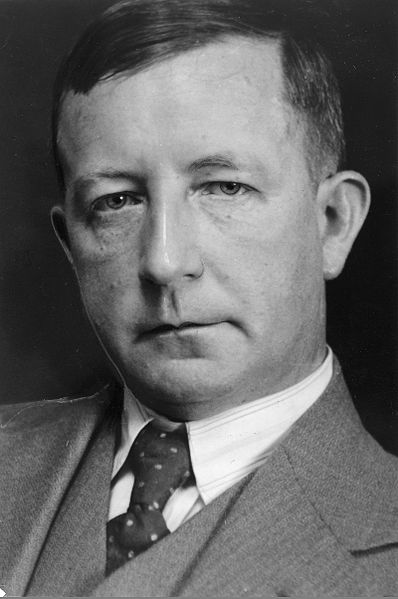
\includegraphics[height=5cm]{images/Skolem.jpg}

\LARGE
Skolem
\end{center}}

\begin{frame}\frametitle{Thoralf Albert Skolem \newline{\small(1887--1963)}}

\ghost{~\hspace{7.3cm}\raisebox{-1cm}{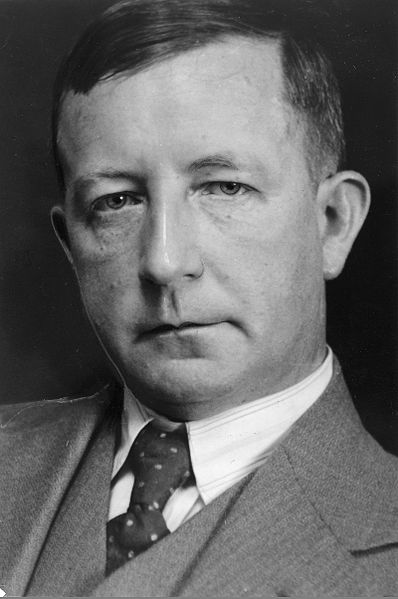
\includegraphics[height=3cm]{images/Skolem.jpg}}}
% Thoralf Albert Skolem (1887--1963)
\begin{itemize}
\item Norwegischer Mathematiker
\item Pionier der mathematischen Logik
\item Wesentliche Beiträge -- zum Teil erst mit großer Verspätung von der Fachwelt wahrgenommen\footnote{Zum Beispiel schlägt er Verbesserungen von Zermelos Mengenlehre vor, fast zeitgleich zu Fraenkel, der dafür berühmt wurde. Auch hätte er fast Gödels Vollständigkeitssatz vor Gödel bewiesen.}
\item Skeptisch gegenüber unendlichen Mengen\footnote{Gödel glaubte, dass diese Abneigung der Grund war, dass Skolem den Vollständigkeitssatz nicht als erster gezeigt hat.}
\end{itemize}\bigskip

(siehe auch Hao Wang, 1996)

\end{frame}

\begin{frame}\frametitle{Skolems Funktionen}

\alert{Eine für uns wesentliche Idee Skolems (1920) ist folgende:}\medskip

\anybox{strongyellow}{Man kann sich existentielle Quantifikation auch
als Auswertung einer Funktion vorstellen, deren Funktionswert das
gesuchte Element ist.}\medskip\pause

\examplebox{Beispiel: Den Satz $\forall x.\exists y.\textsf{hatVater}(x,y)$ ("`Jeder hat einen Vater"') könnte formuliert werden als $\forall x.\textsf{hatVater}(x,\textsf{vater}(x))$. Letzteres ist so zu verstehen:
\begin{itemize}
\item Es gibt eine einstellige Funktion $\textsf{vater}$,
\item welche für jedes Domänenelement den Vater (genauer gesagt "`einen Vater"') des Elements liefert.
\end{itemize}
Daraus folgt insbesondere auch, dass jeder einen Vater hat.
}\medskip

Um das zu formalisieren müssen wir zunächst Funktionssymbole in die Logik einführen.

\end{frame}

\begin{frame}\frametitle{Terme mit Funktionssymbolen}

Prädikatenlogik mit Funktionen verwendet eine erweiterte Signatur:%

\anybox{strongyellow}{\vspace{-1ex}
\begin{itemize}
\item Eine Menge $\Slang{V}$ von \redalert{Variablen} $x$, $y$, $z$, \ldots
\item Eine Menge $\Slang{C}$ von \redalert{Konstanten} $a$, $b$, $c$, \ldots
\item Eine Menge $\Slang{F}$ von \redalert{Funktionssymbolen} $f$, $g$, $h$, \ldots
\item Eine Menge $\Slang{P}$ von \redalert{Prädikatensymbolen} $p$, $q$, $r$, \ldots
\end{itemize}
Jedes Prädikat und jedes Funktionssymbol hat eine \redalert{Stelligkeit} $\geq 0$ (auch \redalert{Arität} genannt). Die Mengen sind abzählbar und disjunkt.}\pause

Mit Funktionssymbolen lassen sich komplexere Terme konstruieren:
\defbox{Ein \redalert{Term} der Prädikatenlogik mit Funktionen ist jeder Ausdruck $t$, der
eine der folgenden rekursiven Bedinungen erfüllt:
\begin{itemize}
\item $t\in\Slang{V}\cup\Slang{C}$, d.h. $t$ ist eine Variable oder eine Konstante
\item $t=f(t_1,\ldots,t_n)$, wobei $f\in\Slang{F}$ ein $n$-stelliges Funktionssymbol ist
und $t_1,\ldots,t_n$ Terme sind.
\end{itemize}}

\end{frame}

\begin{frame}\frametitle{Syntax der Prädikatenlogik mit Funktionen}

Mit dieser Erweiterung können nun Formeln wie gewohnt konstruiert werden:
\bigskip

\defbox{Ein \redalert{Atom} der Prädikatenlogik mit Funktionen ist ein Ausdruck $p(t_1,\ldots,t_n)$
für ein $n$-stelliges Prädikatensymbol $p\in\Slang{P}$ und Terme $t_1,\ldots,t_n$, die Funktionssymbole verwenden dürfen.}\medskip

\defbox{Die Menge der \redalert{prädikatenlogischen Formeln mit Funktionssymbolen} ergibt sich wie bei Prädikatenlogik ohne Funktionen induktiv aus der Menge der Atome unter Verwendung der Operatoren $\neg$, $\wedge$, $\vee$, $\to$, $\leftrightarrow$, $\exists x.$ und $\forall x.$ ($x\in\Slang{V}$).}\medskip

\examplebox{Beispiele:
\begin{itemize}
\item $\forall x.(\textsf{hatBruder}(\textsf{mutter}(x))\to\textsf{hatOheim}(x,\textsf{bruder}(\textsf{mutter}(x))))$
\item $\forall x,y.(\textsf{mutter}(x)\approx\textsf{mutter}(y)\to \textsf{geschwister}(x,y))$
\end{itemize}}

\end{frame}

\begin{frame}\frametitle{Semantik der Prädikatenlogik mit Funktionen} 

Wir müssen nun auf Funktionssymbole interpretieren:

\defbox{Eine \redalert{Interpretation} $\Inter$ der Prädikatenlogik mit Funktionen
ist ein Paar $\tuple{\Delta^\Inter,\cdot^\Inter}$ bestehend aus einer nichtleeren Grundmenge von Elemente $\Delta^\Inter$ (der \redalert{Domäne}) und einer \redalert{Interpretationsfunktion} $\cdot^\Inter$, welche:
\begin{itemize}
\item jede Konstante $a\in\Slang{C}$ auf ein Element $a^\Inter\in\Delta^\Inter$,
\item jedes $n$-stellige Funktionssymbol $f\in\Slang{F}$ auf eine $n$-stellige Funktion $f^\Inter:(\Delta^\Inter)^n\to\Delta^\Inter$ und
\item jedes $n$-stellige Prädikatensymbol $p\in\Slang{P}$ auf eine Relation $p^\Inter\in(\Delta^\Inter)^n$
\end{itemize}
abbildet.
}\medskip

\redalert{Zuweisungen} werden wie zuvor definiert (Abbildungen von Variablen auf Domänenelemente)
\end{frame}

\begin{frame}\frametitle{Formeln mit Funktionssymbolen interpretieren}

Zur Interpretation von Atomen werten wir Funktionsterme gesondert aus:

\defbox{Sei $\Inter$ eine Interpretation und $\Zuweisung$ eine Zuweisung für $\Inter$.
\begin{itemize}
\item Für eine Konstante $c$ definieren wir $c^{\Inter,\Zuweisung}=c^\Inter$
\item Für eine Variable $x$ definieren wir $x^{\Inter,\Zuweisung}=\Zuweisung(x)$
\item Für einen Funktionsterm $t=f(t_1,\ldots,t_n)$ definieren wir $t^{\Inter,\Zuweisung}=f^\Inter(t_1^{\Inter,\Zuweisung},\ldots,t_n^{\Inter,\Zuweisung})$
\end{itemize}
Für ein Atom $p(t_1,\ldots,t_n)$ setzen wir wie gewohnt:
\begin{itemize}
\item $p(t_1,\ldots,t_n)^{\Inter,\Zuweisung}=\mytrue$ wenn $\tuple{t_1^{\Inter,\Zuweisung},\ldots,t_n^{\Inter,\Zuweisung}}\in p^\Inter$ und
\item $p(t_1,\ldots,t_n)^{\Inter,\Zuweisung}=\myfalse$ wenn $\tuple{t_1^{\Inter,\Zuweisung},\ldots,t_n^{\Inter,\Zuweisung}}\notin p^\Inter$.
\end{itemize}
}\bigskip

Wir definieren $\Inter,\Zuweisung\models F$ wie zuvor, rekursiv auf der Struktur
der Formeln.

\end{frame}

\begin{frame}\frametitle{Beispiel}

Gemeinsam mit Gleichheit eignen sich Funktionen gut, um mathematische Operationen auszudrücken.
\bigskip

Die Theorie der kommutativen Monoide ist in Prädikatenlogik mit einem Funktionssymbol $\oplus$ (infix geschrieben) und Gleichheit  wie folgt darstellbar:
\[\begin{array}{r@{}r@{}l}
\forall x,y,z.& ((x\oplus y)\oplus z) &{}\approx(x\oplus (y\oplus z))\\
\forall x,y.& (x\oplus y)& {}\approx(y\oplus x)\\
\forall x.& (x\oplus\Sterm{0})& {}\approx \Sterm{0}
\end{array}\]

Ein mögliches Modell $\Inter$:
\begin{itemize}
\item $\Delta^\Inter=\mathbb{N}$
\item $\Sterm{0}^\Inter=0$
\item ${\oplus^\Inter}={+}$ (Addition über natürlichen Zahlen)
\end{itemize}\bigskip

{\tiny
\emph{Achtung:} Es gibt oft mehr mögliche Modelle als man denkt. Prädikatenlogik eignet sich zur Beschreibung algebraischer Strukturen allgemein, aber nicht zur Beschreibung ganz
spezieller Strukturen wie der natürlichen Zahlen.

}

\end{frame}

\begin{frame}\frametitle{Skolemisierung}
%
% Wir können Skolems Idee nun formal darstellen:

\defbox{Sei $\forall x_1.\cdots\forall x_n.\exists y.F$ eine Formel in Pränexform, bei
der $\exists y$ das erste Vorkommen eines Existenzquantors ist. Die \redalert{Skolemisierung} von $y$ ist die Formel
$\forall x_1.\cdots\forall x_n.F'$, definiert wie folgt:
\begin{itemize}
\item $F'=F\{y\mapsto f(x_1,\ldots,x_n)\}$ entsteht aus $F$, indem man jedes (freie) Vorkommen von $y$ in $F$ durch den \redalert{Skolemterm} $f(x_1,\ldots,x_n)$ ersetzt
\item dabei ist $f$ ein $n$-stelliges Funktionssymbol, das bisher nirgends verwendet wurde, genannt \redalert{Skolemfunktion}.
\end{itemize}
Die Skolemisierung einer Formel in Pränexform erhält man durch Skolemisieren
jeder ihrer existentiell quantifizierten Variablen, von vorn nach hinten.
}\pause

\examplebox{Beispiel: Für die Formel $\forall x.\exists y.\forall z.\exists v.p(x,y,z,v)$ ergibt sich:
\begin{tabular}{rl}
Skolemisierung von $y$: & $\forall x.\forall z.\exists v.p(x,f(x),z,v)$\\
Skolemisierung von $v$: & $\forall x.\forall z.p(x,f(x),z,g(x,z))$
\end{tabular}
}

\end{frame}

\begin{frame}\frametitle{Korrektheit der Skolemisierung}

Skolemisierung führt nicht zu semantisch äquivalenten Formeln:\medskip

\examplebox{Beispiel: Die Formel $\forall x.\exists y.(p(x)\to p(y))$ ist eine Tautologie,
aber ihre Skolemisierung $\forall x.(p(x)\to p(f(y)))$ ist widerlegbar:\\ Sei $\Delta^\Inter\defeq\{\alpha,\beta\}$, $p^\Inter\defeq\{\alpha\}$ sowie $f^\Inter(\delta)\defeq\beta$ für alle $\delta\in\Delta^\Inter$.\\ Dann ist $\Inter\not\models\forall x.(p(x)\to p(f(y)))$, da $\Inter,\{x\mapsto\alpha\}\not\models p(x)\to p(f(y))$.}\medskip\pause

Skolemisierung erhält aber Erfüllbarkeit:\medskip

\theobox{Satz: Eine Formel in Pränexform $F$ ist genau dann erfüllbar, wenn auch die Skolemisierung von $F$ erfüllbar ist.}\medskip

\emph{Anmerkung:} Man kann einen Erfüllbarkeitstest also auf der Skolemisierten Formel ausführen -- das reicht, um logisches Schließen zu implementieren

\end{frame}

\begin{frame}\frametitle{Korrektheit der Skolemisierung: Beweis}

\theobox{Satz: Eine Formel in Pränexform $F$ ist genau dann erfüllbar, wenn auch die Skolemisierung von $F$ erfüllbar ist.}\medskip

\emph{Beweis:} Wir zeigen die Behauptung für die Skolemisierung einer einzelnen Variablen, d.h. die Erfüllbarkeitsäquivalenz von $\forall x_1.\cdots\forall x_n.\exists y.F$ und $\forall x_1.\cdots\forall x_n.F[y\mapsto f(x_1,\ldots,x_n)]$.\\\pause
Dann folgt der Satz durch Induktion über die Zahl der $\exists$.\bigskip\pause

\begin{tabular}{lp{8cm}}
	& $\Inter\models \forall x_1.\cdots\forall x_n.\exists y.F$\\\pause
gdw. & für alle $\delta_1,\ldots, \delta_n\in\Delta^\Inter$ existiert ein $\epsilon\in\Delta^\Inter$, so dass $\Inter,\{x_1\mapsto\delta_1,\ldots,x_n\mapsto \delta_n,y\mapsto\epsilon\}\models F$\\[-2ex]\pause
	& \alert{Wir definieren:} $f^\Inter(\delta_1,\ldots, \delta_n)\defeq\epsilon$ für ein solches $\epsilon$\\\pause
gdw. & für alle $\delta_1,\ldots, \delta_n\in\Delta^\Inter$, so dass\newline $\Inter,\{x_1\mapsto\delta_1,\ldots,x_n\mapsto \delta_n\}\models F\{y\mapsto f(x_1,\ldots,x_n)\}$\\\pause
gdw. & $\Inter\models \forall x_1.\cdots\forall x_n.F\{y\mapsto f(x_1,\ldots,x_n)\}$ \hspace{5cm}\qed
\end{tabular}
% 
% \begin{itemize}
% \item $\Rightarrow$: Laut Semantik bedeutet $\Inter\models x_1.\cdots\forall x_n.\exists y.F$: für alle $\delta_1,\ldots, \delta_n\in\Delta^\Inter$ existiert ein $\epsilon\in\Delta^\Inter$, so dass $\Inter,\{x_i\mapsto\delta_i\mid 1\leq i\leq n\}\{y\mapsto\epsilon\}\models F$.
% \end{itemize}


\end{frame}

\begin{frame}\frametitle{Sind also Funktionen ausdrucksstärker als $\exists$?}
\pause

\redalert{Nein.}
Wir können eine $n$-stellige Funktion $f$ durch ein $(n+1)$-stelliges Prädikat $p_f$
darstellen, z.B. mit folgender Theorie:
\begin{align*}
\forall x_1,\ldots, x_n.\exists y.&p_f(x_1,\ldots,x_n,y)\\
\forall x_1,\ldots, x_n,y,z.&\big((p_f(x_1,\ldots,x_n,y)\wedge p_f(x_1,\ldots,x_n,z))\to y\approx z\big)
\end{align*}\pause

Damit können wir Funktionsterme durch existentiell quantifizierte Variablen mit
entsprechenden Nebenbedingungen ersetzen, z.B.:
\begin{align*}
q(f(x),g(y,z)) &\mapsto \exists v,w.(p_f(x,v)\wedge p_g(y,z,w)\wedge q(v,w))\\
r(g(f(x),y)) &\mapsto \exists v,w.(p_f(x,v)\wedge p_g(v,y,w)\wedge r(w))
\end{align*}\pause
Eine entsprechende Ersetzung kann man bei jedem Atom in einer Formel durchführen. Wir erhalten (ohne Beweis):

\theobox{Satz: Für jede Formel der Prädikatenlogik mit Funktionen gibt es eine erfüllbarkeitsäquivalente Formel ohne Funktionssymbole, welche in linearer Zeit berechnet werden kann.}

\end{frame}

\begin{frame}\frametitle{Zusammenfassung: Funktionen}

Die folgenden Varianten von Prädikatenlogik haben also in gewissem Sinne die \alert{gleiche
Ausdruckstärke:}
\begin{itemize}
\item Prädikatenlogik (ohne Funktionssymbole)
\item Prädikatenlogik mit Funktionssymbolen
\item Prädikatenlogik mit Funktionssymbolen, in Pränexform ohne Existenzquantoren
\end{itemize}
In jeder dieser Logiken kann man zudem wahlweise ein Gleichheitsprädikat hinzufügen
\bigskip\pause

\alert{Vorteile von Skolemfunktionen gegenüber Existenzquantoren:}
\begin{itemize}
\item Es gibt nur noch eine Art von Quantoren
\item Die Abhängigkeiten der existentiell bestimmten Elemente von universell bestimmten Elementen wird explizit in der Syntax dargestellt
\end{itemize}


\end{frame}

\begin{frame}\frametitle{Beispiel: Skolemform}

Wir Skolemisieren das vorige Beispiel:
\[\begin{array}{rl}
& \forall x_1,x_2,x_3,x_4,x_5.\exists x_6,x_7.\\
& \Big(\big((W(x_1)\wedge\neg L(x_1))\vee (L(x_1)\wedge\neg W(x_1))\big)\\
& {}\wedge{}  \big(\neg W(x_2)\vee(W(x_3) \vee L(x_4))\big)\\
& {}\wedge{}  \big(\neg L(x_5)\vee(\neg W(x_6) \wedge \neg L(x_7))\big)\Big)\\\pause
{}\equiv{} & \forall x_1,x_2,x_3,x_4,x_5.\\
& \Big(\big((W(x_1)\wedge\neg L(x_1))\vee (L(x_1)\wedge\neg W(x_1))\big)\\
& {}\wedge{}  \big(\neg W(x_2)\vee(W(x_3) \vee L(x_4))\big)\\
& {}\wedge{}  \big(\neg L(x_5)\vee(\neg W(f_6(x_1,x_2,x_3,x_4,x_5)) \wedge \neg L(f_7(x_1,x_2,x_3,x_4,x_5)))\big)\Big)
\end{array}
\]


\end{frame}

\sectionSlide{Konjunktive Normalform und Klauselform}

\begin{frame}\frametitle{Konjunktive Normalform}

Aus der Aussagelogik kennen wir die folgende Definition:
\bigskip

\defbox{Eine Formel $F$ ist in \redalert{konjunktiver Normalform} (\alert{KNF}) wenn sie 
eine Konjunktion von Disjunktionen von Literalen ist, d.h. wenn sie die Form hat:\\[1ex]
%
\narrowcentering{$(L_{1,1}\vee \ldots\vee L_{1,m_1})\wedge(L_{2,1}\vee \ldots\vee L_{2,m_2})\wedge\ldots
\wedge(L_{n,1}\vee \ldots\vee L_{n,m_n}) $}\\[1ex]
% \narrowcentering{$\bigwedge_{i=1}^n \bigvee_{j=1}^{m_i} L_{i,j}$}\\[1ex]
%
wobei die Formeln $L_{i,j}$ Literale sind. Eine Disjunktion von Literalen heißt \redalert{Klausel}.
}\medskip

(Zur Erinnerung: \redalert{Literale} = negierte oder nicht-negierte Atome)
\bigskip

$\leadsto$ Die gleiche Form kann für den quantorenfreien inneren Teil jeder Formel in Pränexform hergestellt werden.

\end{frame}

\begin{frame}\frametitle{Bilden der KNF}

Wir stellen die KNF in der Prädikatenlogik wie folgt her:
\begin{enumerate}[(1)]
\item Formel bereinigen
\item Bilden der Negationsnormalform
\item Bilden der Pränexform
\item Skolemisieren
\item Erschöpfende Anwendung der folgenden Ersetzung auf Teilformeln im quantorenfreien Teil der Formel:
\begin{align*}
F\vee(G\wedge H) &\mapsto (F\vee G)\wedge (F\vee H)
\end{align*}
\end{enumerate}\pause

\theobox{Satz: Die so aus einer Formel $F$ gebildete KNF ist erfüllbar genau dann wenn $F$ erfüllbar ist.}

\emph{Beweis:} Schritte (1)--(3) liefern sematisch äquivalente Formeln. Schritt (4) liefert eine erfüllbarkeitsäquivalente Formel. Schritt (5) liefert eine zu dieser semantisch äquivalente Formel.\qed\medskip

\emph{Anmerkung:} Man könnte manche der Schritte auch vertauschen.

\end{frame}

\begin{frame}\frametitle{Beispiel: Konjunktive Normalform}

\footnotesize
\[\begin{array}{rl}
& \forall x_1,x_2,x_3,x_4,x_5.\\
& \Big(\hi{2-}{\big((W(x_1)\wedge\neg L(x_1))\vee (L(x_1)\wedge\neg W(x_1))\big)}\\
& {}\wedge{}  \big(\neg W(x_2)\vee(W(x_3) \vee L(x_4))\big)\\
& {}\wedge{}  \big(\neg L(x_5)\vee(\neg W(f_6(x_1,x_2,x_3,x_4,x_5)) \wedge \neg L(f_7(x_1,x_2,x_3,x_4,x_5)))\big)\Big)\\\pause\pause
{}\equiv{} & \forall x_1,x_2,x_3,x_4,x_5.\\
& \Big((W(x_1)\vee L(x_1))\wedge(\neg L(x_1)\vee L(x_1))\\
& {}\wedge (W(x_1)\vee \neg W(x_1))\wedge(\neg L(x_1)\vee \neg W(x_1))\big)\\
& {}\wedge{}  \big(\neg W(x_2)\vee(W(x_3) \vee L(x_4))\big)\\
& {}\wedge{}  \hi{4-}{\big(\neg L(x_5)\vee(\neg W(f_6(x_1,x_2,x_3,x_4,x_5)) \wedge \neg L(f_7(x_1,x_2,x_3,x_4,x_5)))\big)}\Big)\\\pause\pause
{}\equiv{} & \forall x_1,x_2,x_3,x_4,x_5.\\
& \Big((W(x_1)\vee L(x_1))\wedge(\neg L(x_1)\vee L(x_1))\\
& {}\wedge (W(x_1)\vee \neg W(x_1))\wedge(\neg L(x_1)\vee \neg W(x_1))\big)\\
& {}\wedge{}  \big(\neg W(x_2)\vee(W(x_3) \vee L(x_4))\big)\\
& {}\wedge{}  (\neg L(x_5)\vee\neg W(f_6(x_1,x_2,x_3,x_4,x_5))) \wedge (\neg L(x_5)\vee\neg L(f_7(x_1,x_2,x_3,x_4,x_5)))\Big)
\end{array}
\]


\end{frame}


\begin{frame}\frametitle{Klauselform}

Die \redalert{Klauselform} ist eine vereinfachte Schreibweise der KNF:
\begin{itemize}
\item Allquantoren werden weggelassen
\item Klauseln werden als Mengen von Literalen geschrieben
\item Konjunktionen von Klauseln werden als Mengen von Mengen von Literalen geschrieben
\end{itemize}

\examplebox{Beispiel: Unser Beispiel kann damit wie folgt geschrieben werden:\\[-2.5ex]
%
\[\begin{array}{rl}
\{& \{W(x_1), L(x_1)\},\\
& \{\neg L(x_1), L(x_1)\},\\
& \{W(x_1), \neg W(x_1)\},\\
& \{\neg L(x_1), \neg W(x_1)\},\\
& \{\neg W(x_2), W(x_3), L(x_4)\},\\
& \{\neg L(x_5),\neg W(f_6(x_1,x_2,x_3,x_4,x_5))\},\\
& \{\neg L(x_5),\neg L(f_7(x_1,x_2,x_3,x_4,x_5))\}\quad\}
\end{array}
\]
}

\end{frame}



% Entailment
% - Probleme, Reduktionen
% - Unentscheidbarkeit
% Model Checking
% - PSpace-Completeness
% Equality
% - Simulation (sat. preservation)
% Function symbols
% - Simulation (sat. preservation)



\begin{frame}\frametitle{Zusammenfassung und Ausblick}

Die Pränexform entsteht durch einfaches Vorziehen der Quantoren aus einer NNF\bigskip

Funktionen liefern keine zusätzliche Ausdrucksstärke, aber sie helfen bei der
Normalisierung von Formeln, da man existentielle Variablen durch Funktionsterme ersetzten kann (Skolemform)
\bigskip

Konjunktive Normalform und Klauselform werden wie in der Aussagenlogik gebildet
\bigskip

\anybox{yellow}{
Was erwartet uns als nächstes?
\begin{itemize}
\item Herbrand, genialer Mathematiker aber unglücklicher Bergsteiger
\item Unifikation und Resolution
\item Logik über endlichen Modellen und ihre praktische Anwendung
\end{itemize}
}

\end{frame}




\begin{frame}[t]\frametitle{Literatur und Bildrechte}

\alert{Literatur}\bigskip

\begin{itemize}
\item Thoralf A. Skolem: \emph{Logisch-kombinatorische Untersuchungen über die Erfüllbarkeit und Beweisbarkeit mathematischen Sätze nebst einem Theoreme über dichte Mengen.} Videnskapsselskapets Skrifter. I. Mat.-naturv Klasse, 1920, No. 4. Kristiania 1920.
\item Hao Wang: \emph{Skolem and Gödel.} Nordic Journal of Philosophical Logic, Vol. 1, No. 2, pp. 119–132. \url{http://www.hf.uio.no/ifikk/forskning/publikasjoner/tidsskrifter/njpl/vol1no2/skogod.pdf}
\end{itemize}

\bigskip

\alert{Bildrechte}\bigskip

Folie \ref{frame_skolem}: Fotografie, 1930er (heute Oslo Museum, Inventarnummer OB.F06426c), gemeinfrei

\end{frame}


\end{document}